\documentclass[11pt,a4paper]{article}

\usepackage[utf8]{inputenc}
\usepackage[T1]{fontenc}
\usepackage{amsmath}
\usepackage{booktabs}
\usepackage{graphicx}
\usepackage{siunitx}
\usepackage{tabularx}
\usepackage{array}
\usepackage{caption}
\usepackage{subcaption}
\usepackage{xcolor}
\usepackage{tikz}
\usetikzlibrary{arrows.meta,positioning,fit,calc}
\usepackage[hidelinks]{hyperref}

\sisetup{detect-weight=true, detect-family=true}
\setlength{\emergencystretch}{2em}
\graphicspath{{../}}

\title{CNN-based Severity Classification of Diabetic Retinopathy with Explainability Analysis}
\author{Yassine Abderrazik, Mark Salloum, Adel Atzouza,\\
Musab Sivrikaya, Ozeir Moradi\\
Rotterdam University of Applied Sciences\\
Wijnhaven 107, Rotterdam, 3011WN, The Netherlands}
\date{}

\begin{document}
\maketitle

\section*{Highlights}
\begin{itemize}
  \item A reproducible APTOS~2019 diabetic retinopathy grading pipeline was implemented using green-channel preprocessing, ImageNet-pretrained EfficientNet backbones, and validation-QWK checkpointing.
  \item EfficientNetB3 achieved the strongest held-out performance among the tested variants, reaching QWK \(0.8908\), accuracy \(0.8005\), and macro ROC-AUC \(0.9320\).
  \item SMOTE oversampling and ordinal regression were evaluated as ablations but did not improve the final held-out QWK over the selected EfficientNetB3 model.
  \item Grad-CAM, Grad-CAM++, and Score-CAM were used as qualitative explainability tools and revealed both plausible retinal attention and border/corner artefact reliance.
\end{itemize}

\begin{abstract}
Diabetic retinopathy (DR) is a leading cause of preventable vision loss, and automated grading of retinal fundus images can support scalable screening. However, benchmark accuracy alone is insufficient for clinical trust because model errors, class imbalance, and non-clinical image artefacts may remain hidden. This study develops and evaluates a reproducible convolutional-neural-network pipeline for five-class DR severity grading on the APTOS~2019 fundus image dataset. Images were standardised using black-border cropping, aspect-ratio-preserving resizing, green-channel extraction, CLAHE, median filtering, and float normalisation. ImageNet-pretrained EfficientNetB0, EfficientNetB1, and EfficientNetB3 backbones were compared using class-weighted softmax training and validation quadratic weighted kappa (QWK) checkpointing. Additional ablations evaluated SMOTE oversampling and an ordinal-regression head with validation-tuned thresholds. The selected EfficientNetB3 model achieved the best held-out test QWK (\(0.8908\)), accuracy (\(0.8005\)), macro specificity (\(0.9530\)), and macro ROC-AUC (\(0.9320\)). It improved mild and proliferative DR sensitivity compared with the EfficientNetB0 baseline, but severe DR sensitivity decreased from \(0.6471\) to \(0.3529\), indicating an important minority-class failure mode. Grad-CAM, Grad-CAM++, and Score-CAM were generated for the selected model. The resulting heatmaps showed some plausible retinal attention, but recurring activation near image borders and corners suggests that the model may also exploit non-pathological acquisition artefacts. The pipeline therefore demonstrates strong grading performance on APTOS~2019 while highlighting the need for external validation, lesion-level annotations, and further work on severe-grade recall and explanation faithfulness.
\end{abstract}

\noindent\textbf{Keywords:} Diabetic retinopathy; EfficientNet; APTOS 2019; quadratic weighted kappa; Grad-CAM; Score-CAM; explainable AI; class imbalance.

\section{Introduction}
Diabetic retinopathy (DR) is a chronic microvascular complication of diabetes mellitus and one of the leading causes of preventable blindness among working-age adults worldwide \cite{teo2021}. Its clinical relevance is not limited to detection of disease presence: DR severity is graded on an ordinal scale, and each stage implies a different level of follow-up urgency and clinical intervention \cite{etdrs1991}. Automated systems must therefore distinguish between no DR, mild, moderate, severe, and proliferative DR rather than only detecting referable disease.

Deep learning has shown strong performance in retinal-image analysis, particularly when convolutional neural networks are pre-trained on large-scale natural image datasets and fine-tuned on fundus images \cite{gulshan2016,ting2017}. Nevertheless, several barriers limit the direct clinical interpretation of such systems. First, DR datasets are strongly imbalanced, with severe grades represented by relatively few examples \cite{atwany2022}. Second, high aggregate performance can mask clinically important minority-grade errors. Third, visual explanation methods can produce plausible heatmaps without necessarily proving that a model uses lesion-level evidence \cite{ayhan2022}. These limitations are central in a medical-screening setting, where a model can appear accurate while still relying on acquisition artefacts, retinal borders, or other non-pathological cues.

This study addresses these issues by developing and evaluating a reproducible DR severity-grading pipeline on the APTOS~2019 dataset. The study focuses on three research questions: how effectively CNN-based approaches perform five-class DR grading; to what extent visual explanation methods highlight clinically plausible retinal regions; and how class-imbalance strategies affect grading performance and explanation quality. In contrast to broader planned extensions, the implemented scope is intentionally narrow and evidence-based: APTOS~2019 is the only dataset used, EfficientNetB0/B1/B3 backbones are compared, SMOTE and ordinal regression are treated as separate ablations, and Grad-CAM, Grad-CAM++, and Score-CAM are interpreted qualitatively rather than as lesion-mask validation.

The contributions of this work are fourfold. First, we implement an end-to-end preprocessing, training, and evaluation pipeline with explicit array and model-input contracts. Second, we compare EfficientNetB0, EfficientNetB1, and EfficientNetB3 under a fixed class-weighted training recipe. Third, we evaluate imbalance and ordinal-label ablations using SMOTE and regression-threshold tuning. Fourth, we audit the selected model with three class-activation methods and document both plausible attention patterns and failure modes.

\section{Related Work}
\subsection{Deep Learning for DR Grading}
Deep learning-based DR grading has progressed rapidly since large-scale convolutional models demonstrated expert-level performance for referable DR detection in retinal fundus photographs \cite{gulshan2016,ting2017}. Subsequent studies have applied ResNet, DenseNet, Inception, VGG, EfficientNet, and ensemble architectures to either binary DR screening or multi-class severity grading \cite{atwany2022}. Transfer learning is particularly common because labelled medical-image datasets are typically much smaller than general-purpose image corpora.

EfficientNet is well suited to this setting because it scales network depth, width, and resolution using a compound coefficient, offering a favourable trade-off between capacity and computational cost \cite{efficientnet}. In DR grading, EfficientNet variants have been used both as compact baselines and as higher-capacity backbones \cite{chetoui2020,vijayan2023}. The proposal for this work therefore identified EfficientNetB0, EfficientNetB1, and EfficientNetB3 as a useful complexity progression: B0 provides an efficient baseline, B1 offers moderate capacity, and B3 tests whether additional representational power improves ordinal severity grading.

\subsection{Explainability in Medical Imaging}
Class-activation methods such as Grad-CAM are frequently used to visualise spatial evidence behind CNN predictions \cite{gradcam}. In medical imaging, these methods are attractive because they can be overlaid directly on clinical images and inspected by domain experts. However, saliency maps should not be treated as clinical proof by default. Prior work has shown that explanation quality depends on both architecture and method, and that visually plausible heatmaps may still fail to align consistently with clinically meaningful lesions \cite{ayhan2022}.

This distinction is important for DR grading. The International Clinical DR scale depends on lesion patterns such as microaneurysms, haemorrhages, exudates, venous beading, intraretinal microvascular abnormalities, and neovascularisation. A heatmap over a fundus photograph is clinically useful only if it supports a plausible connection between image regions and grade-defining pathology. Without pixel-level lesion masks or clinician scoring, explanation analysis remains qualitative and should be framed as model auditing rather than lesion-level validation.

\subsection{Class Imbalance in DR Datasets}
Class imbalance is a persistent problem in DR datasets. No-DR and moderate-DR images often dominate, while severe and proliferative cases are less frequent \cite{atwany2022}. A model trained naively on such data can optimise aggregate accuracy while under-detecting clinically important minority grades. Common strategies include class-weighted loss functions, weighted sampling, data augmentation, and oversampling methods such as SMOTE \cite{smote,shorten2019}.

SMOTE is attractive in tabular feature spaces because it synthesises minority examples by interpolating between neighbours. In pixel-space medical imaging, however, synthetic interpolation can produce unrealistic structures or blur clinically meaningful detail. For that reason, this study treats SMOTE as a separate ablation rather than as part of the canonical preprocessing pipeline, and evaluates it using held-out test QWK and per-class sensitivity rather than accuracy alone.

\section{Methodology}
Figure~\ref{fig:research-pipeline} summarises the implemented research
pipeline. The figure distinguishes fixed data preparation from experimental
branches and from the final evaluation and explainability audit. This
separation is important because only the training split is modified in the
SMOTE ablation, while validation and held-out test splits remain unchanged for
all experiments.

\begin{figure}[t]
  \centering
  \resizebox{\textwidth}{!}{%
  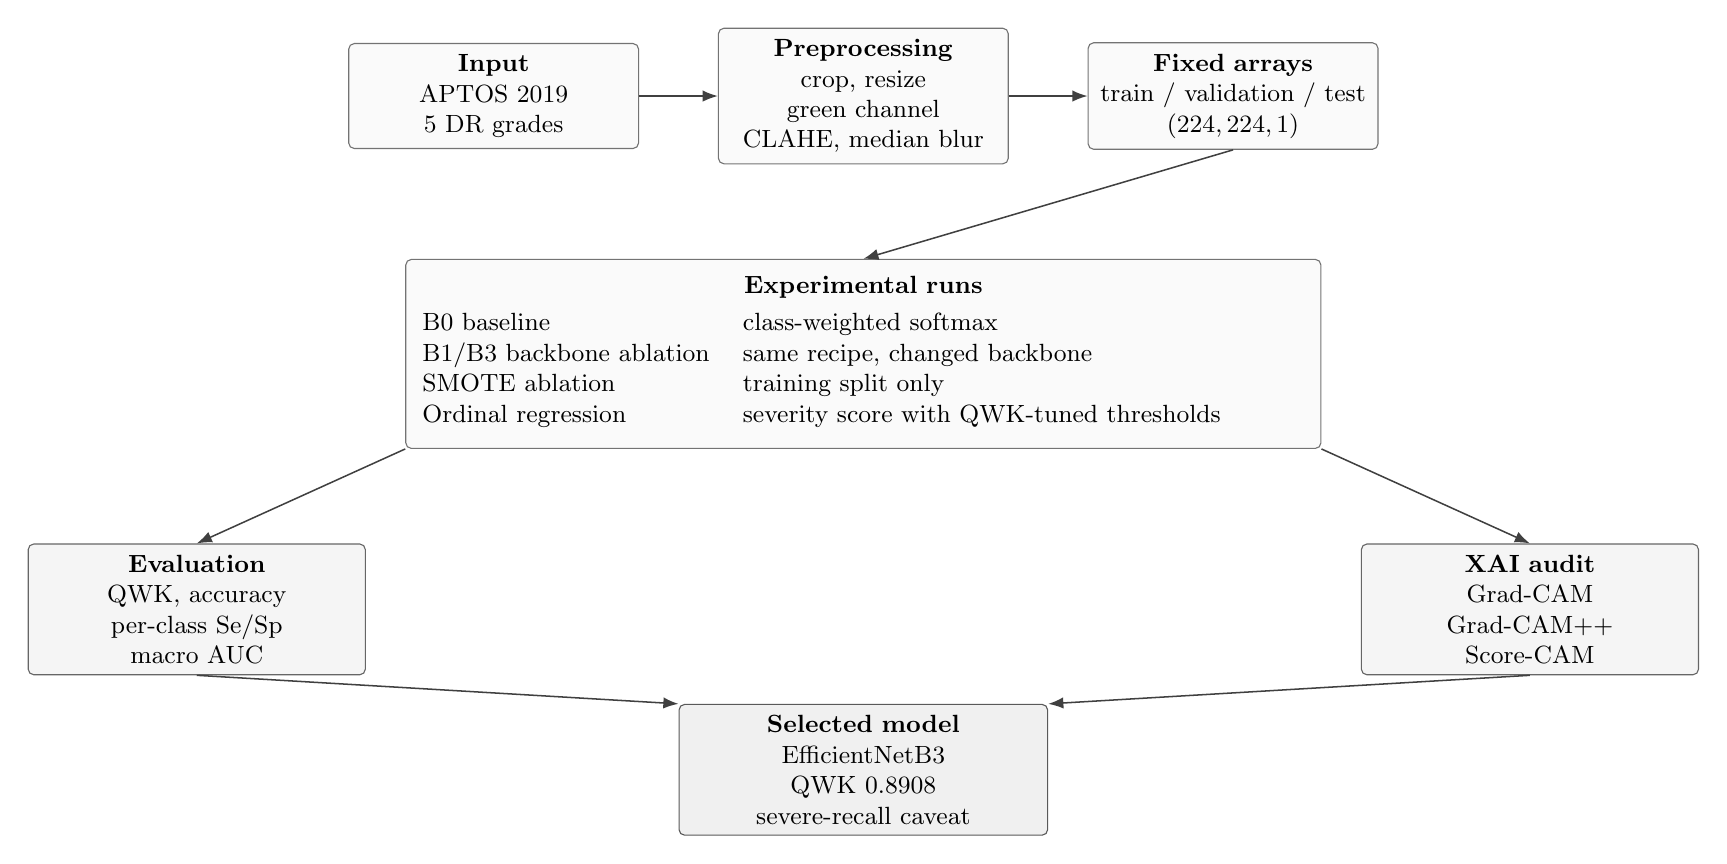
\begin{tikzpicture}[
    font=\small,
    node distance=9mm and 10mm,
    block/.style={draw=black!55, rounded corners=2pt, align=center,
      text width=34mm, minimum height=11mm, inner sep=4pt, fill=black!2},
    wide/.style={draw=black!55, rounded corners=2pt, align=left,
      text width=112mm, minimum height=24mm, inner sep=6pt, fill=black!2},
    output/.style={draw=black!60, rounded corners=2pt, align=center,
      text width=40mm, minimum height=12mm, inner sep=4pt, fill=black!4},
    selected/.style={draw=black!65, rounded corners=2pt, align=center,
      text width=44mm, minimum height=13mm, inner sep=4pt, fill=black!6},
    arrow/.style={-Latex, line width=0.55pt, black!75}
  ]
    \node[block] (data) {\textbf{Input}\\APTOS 2019\\5 DR grades};
    \node[block, right=of data] (prep) {\textbf{Preprocessing}\\crop, resize\\green channel\\CLAHE, median blur};
    \node[block, right=of prep] (splits) {\textbf{Fixed arrays}\\train / validation / test\\\((224,224,1)\)};

    \node[wide, below=12mm of prep] (experiments) {%
      \centering\textbf{Experimental runs}\\[1mm]
      \begin{tabular}{@{}ll@{}}
        B0 baseline & class-weighted softmax \\
        B1/B3 backbone ablation & same recipe, changed backbone \\
        SMOTE ablation & training split only \\
        Ordinal regression & severity score with QWK-tuned thresholds
      \end{tabular}
    };

    \node[output, below left=12mm and 5mm of experiments] (metrics)
      {\textbf{Evaluation}\\QWK, accuracy\\per-class Se/Sp\\macro AUC};
    \node[output, below right=12mm and 5mm of experiments] (xai)
      {\textbf{XAI audit}\\Grad-CAM\\Grad-CAM++\\Score-CAM};
    \coordinate (auditmid) at ($(metrics)!0.5!(xai)$);
    \node[selected, below=12mm of auditmid] (selected)
      {\textbf{Selected model}\\EfficientNetB3\\QWK \(0.8908\)\\severe-recall caveat};

    \draw[arrow] (data) -- (prep);
    \draw[arrow] (prep) -- (splits);
    \draw[arrow] (splits.south) -- (experiments.north);
    \draw[arrow] (experiments.south west) -- (metrics.north);
    \draw[arrow] (experiments.south east) -- (xai.north);
    \draw[arrow] (metrics.south) -- (selected.north west);
    \draw[arrow] (xai.south) -- (selected.north east);
  \end{tikzpicture}
  }
  \caption{Implemented DR grading research pipeline. Fixed preprocessing and
  fixed validation/test splits are shared by all experiments. The selected
  EfficientNetB3 run is chosen by held-out QWK, while the severe-grade recall
  drop and XAI border attention are treated as failure modes.}
  \label{fig:research-pipeline}
\end{figure}

\subsection{Datasets}
This study uses the APTOS~2019 Blindness Detection dataset \cite{aptos2019}. Each image is labelled on a five-class DR severity scale: grade 0 (no DR), grade 1 (mild), grade 2 (moderate), grade 3 (severe), and grade 4 (proliferative DR). The current implementation uses \num{2930} training images, \num{366} validation images, and \num{366} held-out test images. These splits are kept fixed across all experiments.

\begin{table}[t]
  \centering
  \caption{APTOS~2019 class distribution used in this study.}
  \label{tab:class-distribution}
  \begin{tabular}{lrrrrrr}
    \toprule
    Split & Grade 0 & Grade 1 & Grade 2 & Grade 3 & Grade 4 & Total \\
    \midrule
    Train & 1434 & 300 & 808 & 154 & 234 & 2930 \\
    Validation & 172 & 40 & 104 & 22 & 28 & 366 \\
    Test & 199 & 30 & 87 & 17 & 33 & 366 \\
    \bottomrule
  \end{tabular}
\end{table}

The distribution in Table~\ref{tab:class-distribution} shows the imbalance typical of DR grading: no-DR images form the largest group, whereas severe DR is the smallest class in all splits. This motivates per-class evaluation and class-weighted training.

\subsection{Preprocessing}
The preprocessing pipeline standardises heterogeneous fundus photographs while preserving the natural validation and test distributions. Images are converted to RGB, near-black camera borders are cropped, and the retinal field is resized to \(224 \times 224\) using aspect-ratio-preserving zero padding. The green channel is then extracted because vascular and haemorrhagic structures generally have stronger contrast in this channel than in the red or blue channels. Contrast-Limited Adaptive Histogram Equalisation (CLAHE) is applied with clip limit 2.0 and an \(8 \times 8\) tile grid \cite{pizer1987,alwakid2023}, followed by median filtering with kernel size 3 and conversion to \texttt{float32} values in \([0,1]\).

The saved image-array contract is \((N,224,224,1)\). The model graph, not the preprocessing output, handles compatibility with ImageNet-pretrained EfficientNet models: the one-channel input is scaled to the range expected by Keras EfficientNet and repeated into three channels inside the network. This separation prevents accidental double-normalisation and makes the data contract explicit.

\begin{figure}[t]
  \centering
  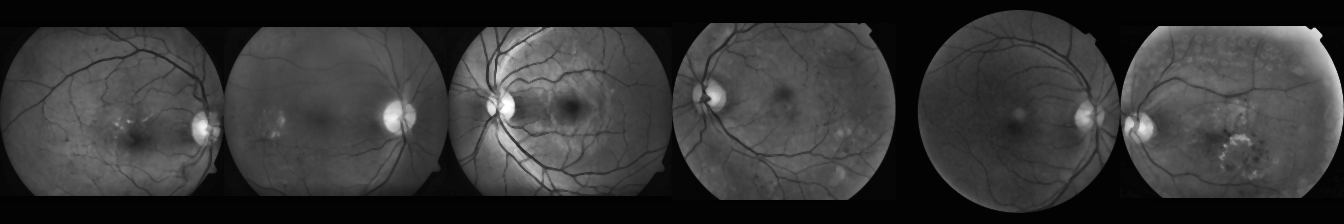
\includegraphics[width=\textwidth]{data/preprocessed/_samples/train_samples.png}
  \caption{Examples from the preprocessed training split. Images are stored as one-channel green-channel tensors after border cropping, aspect-ratio-preserving resizing, CLAHE, median filtering, and normalisation.}
  \label{fig:preprocessed-samples}
\end{figure}

\subsection{Model Architecture and Training}
All classification models use an ImageNet-pretrained EfficientNet backbone with the original classification head removed. The custom head consists of global average pooling, batch normalisation, dropout, a dense layer with 1024 hidden units, a second dropout layer, and a five-unit softmax output. EfficientNetB0, EfficientNetB1, and EfficientNetB3 are evaluated using the same input contract and training recipe, except that EfficientNetB3 uses a smaller batch size due to higher memory requirements.

Training uses class weights derived from the training-label distribution. The model is fine-tuned with the backbone unfrozen, while batch-normalisation layers inside the backbone remain effectively stabilised through the transfer-learning setup. Model selection is based on validation QWK, with early stopping, model checkpointing, and learning-rate reduction also monitoring validation QWK. The held-out test set is evaluated only after training has selected the best validation checkpoint.

Two additional ablations are evaluated. The SMOTE ablation uses an oversampled training array while leaving validation and test splits unchanged. The ordinal-regression ablation replaces the softmax classifier with a single linear severity-score output trained with a regression loss; validation predictions are converted back to five classes using ordered thresholds selected to maximise validation QWK.

\subsection{Evaluation methods}
Evaluation is aligned with the ordinal and imbalanced nature of DR grading. Quadratic weighted kappa is the primary metric because it penalises mistakes according to their ordinal distance. Accuracy is reported as a secondary aggregate metric but is not sufficient on its own. Per-class sensitivity and specificity are reported to expose grade-specific failure modes, and macro ROC-AUC is used as a supplementary one-vs-rest discriminability metric. Confusion matrices are used to inspect error patterns across severity grades.

\begin{table}[t]
  \centering
  \caption{Evaluation framework used in the implemented study.}
  \label{tab:evaluation-framework}
  \begin{tabularx}{\textwidth}{p{1.2cm}p{3.2cm}X}
    \toprule
    RQ & Dimension & Instruments \\
    \midrule
    RQ1 & Classification performance & QWK, accuracy, per-class sensitivity/specificity, macro ROC-AUC, and confusion matrix. \\
    RQ2 & Explainability quality & Qualitative review of Grad-CAM, Grad-CAM++, and Score-CAM heatmaps, including failure-mode inspection. \\
    RQ3 & Imbalance sensitivity & Comparison of baseline, SMOTE, ordinal regression, and backbone ablations using QWK and per-class sensitivity. \\
    \bottomrule
  \end{tabularx}
\end{table}

\subsection{Explainability Methods}
Grad-CAM, Grad-CAM++, and Score-CAM are applied to the selected EfficientNetB3 model. Grad-CAM uses gradients flowing into the final convolutional activation to weight spatial feature maps \cite{gradcam}. Grad-CAM++ modifies the weighting scheme to emphasise spatially important positive gradients. Score-CAM avoids gradients by masking the input image with upsampled activation maps and weighting those masks by the model's class scores. To keep Score-CAM computationally tractable for EfficientNet feature maps, the implementation uses the top activated channels rather than all channels.

Before heatmaps are generated, the Grad-CAM model path is validated by checking that the rebuilt explanation model produces predictions equivalent to the original saved model. This guards against a common implementation error in which explanations are generated from a graph that no longer exactly matches the trained classifier.

\subsection{Explainability Evaluation Protocol}
The explainability evaluation is qualitative. Heatmaps are generated per severity grade, and examples are inspected for whether attention falls on plausible retinal regions or on artefacts such as borders, padding, camera field edges, or the optic disc. Because no lesion-level masks are used in the implemented study, the paper does not report pointing-game accuracy, IoU, or quantitative lesion-overlap scores. Instead, the explanation outputs are treated as model-auditing evidence: they can reveal plausible behaviour and failure modes, but they cannot prove lesion-level clinical faithfulness.

\section{Experiments and Results}
\subsection{Experimental Setup}
All experiments use the same APTOS~2019 splits and preprocessing contract. The primary baseline is a class-weighted EfficientNetB0 softmax model. Ablations include SMOTE oversampling, ordinal regression with threshold optimisation, EfficientNetB1, and EfficientNetB3. Each run writes artifacts to a separate directory so that results are not overwritten. The selected run is EfficientNetB3 because it achieves the highest held-out test QWK.

\subsection{Classification Performance}
\begin{table}[t]
  \centering
  \caption{Held-out test performance across all model and imbalance ablations.}
  \label{tab:main-results}
  \resizebox{\textwidth}{!}{%
  \begin{tabular}{lrrrrr}
    \toprule
    Run & QWK & Accuracy & Macro Se & Macro Sp & Macro AUC \\
    \midrule
    EfficientNetB0 baseline & 0.8655 & 0.7842 & 0.6431 & 0.9492 & 0.9204 \\
    SMOTE & 0.8629 & 0.7869 & 0.5997 & 0.9483 & 0.9083 \\
    Ordinal regression & 0.8037 & 0.6612 & 0.4520 & 0.9165 & 0.8032 \\
    EfficientNetB1 & 0.8595 & 0.7678 & 0.6154 & 0.9449 & 0.9265 \\
    EfficientNetB3 & \textbf{0.8908} & \textbf{0.8005} & 0.6402 & \textbf{0.9530} & \textbf{0.9320} \\
    \bottomrule
  \end{tabular}
  }
\end{table}

Table~\ref{tab:main-results} shows that EfficientNetB3 is the strongest model on the primary metric. It improves QWK by 0.0253 over the EfficientNetB0 baseline and also improves accuracy, macro specificity, and macro AUC. Macro sensitivity is slightly lower than B0 because of a substantial decrease in severe-grade recall.

\begin{table}[t]
  \centering
  \caption{Per-class sensitivity for the main experimental runs.}
  \label{tab:per-class-sensitivity}
  \resizebox{\textwidth}{!}{%
  \begin{tabular}{lrrrrr}
    \toprule
    Run & Grade 0 & Grade 1 & Grade 2 & Grade 3 & Grade 4 \\
    \midrule
    EfficientNetB0 baseline & 0.9598 & 0.5333 & 0.6207 & 0.6471 & 0.4545 \\
    SMOTE & 0.9648 & 0.2667 & 0.7241 & 0.5882 & 0.4545 \\
    Ordinal regression & 0.8392 & 0.3333 & 0.6437 & 0.3529 & 0.0909 \\
    EfficientNetB1 & 0.9548 & 0.5333 & 0.5747 & 0.5294 & 0.4848 \\
    EfficientNetB3 & \textbf{0.9648} & \textbf{0.6333} & 0.6437 & 0.3529 & \textbf{0.6061} \\
    \bottomrule
  \end{tabular}
  }
\end{table}

The per-class sensitivities in Table~\ref{tab:per-class-sensitivity} clarify the trade-off behind the B3 selection. B3 improves mild and proliferative DR recall, two clinically relevant minority categories, but severe DR recall decreases from 0.6471 for B0 to 0.3529. This is the most important failure mode of the selected model and is therefore not hidden behind the higher aggregate QWK.

\begin{figure}[t]
  \centering
  
\includegraphics[width=\textwidth]{artifacts/b3/figures/confusion_matrix.png}
  \caption{EfficientNetB3 held-out test confusion matrix. The row-normalised panel shows per-grade recall and highlights the severe-grade limitation.}
  \label{fig:b3-confusion}
\end{figure}

\begin{figure}[t]
  \centering
  
\includegraphics[width=0.90\textwidth]{artifacts/b3/figures/per_class_metrics.png}
  \caption{Per-class sensitivity, specificity, and one-vs-rest AUC for the selected EfficientNetB3 model.}
  \label{fig:b3-per-class}
\end{figure}

\begin{figure}[t]
  \centering
  
\includegraphics[width=\textwidth]{artifacts/b3/figures/training_curves.png}
  \caption{EfficientNetB3 training curves reconstructed from the MLflow metric history. The best validation-QWK checkpoint is selected for held-out test evaluation.}
  \label{fig:b3-training}
\end{figure}

\subsection{Explainability Results}
Figure~\ref{fig:b3-xai} compares the three explanation methods on one correctly classified example per grade. Score-CAM generally produces broader maps, while Grad-CAM++ is visually sharper. Some highlighted regions overlap the retinal field and appear clinically plausible, especially for moderate and proliferative cases. However, Grad-CAM and Grad-CAM++ also show recurring activation near the image border or upper-right corner. This pattern is not consistent with lesion-level reasoning and suggests that the selected model may partly rely on acquisition or preprocessing artefacts.

\begin{figure}[t]
  \centering
  \begin{subfigure}{\textwidth}
    \centering
    \includegraphics[width=\textwidth]{artifacts/b3/figures/gradcam_summary.png}
    \caption{Grad-CAM}
  \end{subfigure}
  \vspace{0.5em}
  \begin{subfigure}{\textwidth}
    \centering
    
\includegraphics[width=\textwidth]{artifacts/b3/figures/gradcampp_summary.png}
    \caption{Grad-CAM++}
  \end{subfigure}
  \vspace{0.5em}
  \begin{subfigure}{\textwidth}
    \centering
    
\includegraphics[width=\textwidth]{artifacts/b3/figures/scorecam_summary.png}
    \caption{Score-CAM}
  \end{subfigure}
  \caption{Qualitative explainability comparison for the selected EfficientNetB3 model. Heatmaps are useful for auditing, but corner and border activations prevent lesion-level claims.}
  \label{fig:b3-xai}
\end{figure}

\subsection{Impact of Class Imbalance Handling}
The imbalance experiments show that changing the training distribution is not automatically beneficial. SMOTE slightly improves accuracy but reduces QWK and macro sensitivity compared with B0. Most importantly, mild DR recall drops from 0.5333 to 0.2667. Ordinal regression is theoretically attractive because DR grades are ordered, but the implemented regression head generalises poorly on the held-out test set, reaching QWK 0.8037 and proliferative recall 0.0909. The strongest result comes from a larger class-weighted backbone rather than synthetic oversampling or a different output formulation.

\section{Discussion}
The primary result is that EfficientNetB3 outperforms the lower-capacity backbones and the imbalance/ordinal ablations on held-out QWK. This supports the proposal's hypothesis that comparing EfficientNet variants can reveal an accuracy-capacity trade-off. B1 did not improve over B0 on the test set, but B3 did, indicating that additional capacity can help when combined with a stable preprocessing and class-weighted training pipeline.

At the same time, the results show why QWK must be interpreted with per-class metrics. B3 improves the ordinal agreement score and raises proliferative DR sensitivity, but severe DR sensitivity is lower than B0. The severe class has only 17 test examples, making this estimate statistically fragile, but the clinical implication is still important: a model selected purely on QWK may under-detect a small but clinically serious category. For a screening support system, this failure mode would require further mitigation before deployment.

The SMOTE ablation also illustrates a practical limitation. Although oversampling is commonly proposed for imbalanced datasets, pixel-space interpolation can alter retinal structure and does not guarantee better minority-grade learning. In this study, SMOTE does not improve final QWK and substantially hurts mild DR recall. Class-weighted training with real images is therefore preferable for the current pipeline.

The ordinal-regression ablation addresses the ordered nature of DR labels but performs worse than softmax classification. This does not invalidate ordinal modelling in general; rather, it shows that the simple single-output regression head and validation-threshold tuning used here are insufficient for this dataset and training setup. More specialised ordinal losses or cumulative-link formulations may be more appropriate future work.

The explainability results should be interpreted conservatively. The generated heatmaps provide useful audit information, especially when they reveal attention outside clinically meaningful regions. Recurrent corner and border activation suggests possible reliance on padding, camera framing, or other acquisition artefacts. Therefore, this paper does not claim lesion-level validation. Without IDRiD-style lesion masks or clinician annotation of heatmap quality, the XAI component remains qualitative failure-mode analysis.

Several limitations remain. The study uses APTOS~2019 only, so cross-dataset generalisation to EyePACS, Messidor, or local clinical images is unknown. The held-out test set is internal to the same dataset source rather than an external validation cohort. The severe class is small, making grade-specific recall unstable. Finally, no prospective clinical evaluation, calibration analysis, or clinician reader study is performed.

\section{Conclusion}
This study developed a reproducible CNN-based pipeline for five-class diabetic retinopathy grading on APTOS~2019. The implemented experiments compared EfficientNetB0, EfficientNetB1, EfficientNetB3, SMOTE oversampling, and ordinal regression under a fixed preprocessing and evaluation protocol. EfficientNetB3 achieved the best held-out QWK (\(0.8908\)) and is the current selected model, but its reduced severe-grade sensitivity is a central limitation. Grad-CAM, Grad-CAM++, and Score-CAM provided qualitative insight into model behaviour and revealed both plausible retinal attention and spurious border/corner activation. Future work should prioritise external validation, lesion-mask or clinician-based explanation evaluation, calibration, and targeted methods for improving severe-grade sensitivity without sacrificing the gains in QWK and proliferative DR recall.

\begin{thebibliography}{18}

\bibitem{teo2021}
Z. L. Teo, Y.-C. Tham, M. Yu, M. L. Chee, T. H. Rim, N. Cheung, M. M. Bikbov, Y. X. Wang, Y. Tang, Y. Lu, I. Y. Wong, D. S. W. Ting, G. S. W. Tan, J. B. Jonas, C. Sabanayagam, T. Y. Wong, and C.-Y. Cheng, ``Global prevalence of diabetic retinopathy and projection of burden through 2045: systematic review and meta-analysis,'' \emph{Ophthalmology}, vol. 128, no. 11, pp. 1580--1591, 2021.

\bibitem{etdrs1991}
Early Treatment Diabetic Retinopathy Study Research Group, ``Grading diabetic retinopathy from stereoscopic color fundus photographs: ETDRS report number 10,'' \emph{Ophthalmology}, vol. 98, no. 5 Suppl., pp. 786--806, 1991.

\bibitem{gulshan2016}
V. Gulshan, L. Peng, M. Coram, M. C. Stumpe, D. Wu, A. Narayanaswamy, S. Venugopalan, K. Widner, T. Madams, J. Cuadros, R. Kim, R. Raman, P. C. Nelson, J. L. Mega, and D. R. Webster, ``Development and validation of a deep learning algorithm for detection of diabetic retinopathy in retinal fundus photographs,'' \emph{JAMA}, vol. 316, no. 22, pp. 2402--2410, 2016.

\bibitem{ting2017}
D. S. W. Ting \emph{et al.}, ``Development and validation of a deep learning system for diabetic retinopathy and related eye diseases using retinal images from multiethnic populations with diabetes,'' \emph{JAMA}, vol. 318, no. 22, pp. 2211--2223, 2017.

\bibitem{atwany2022}
M. Z. Atwany, A. H. Sahyoun, and M. Yaqub, ``Deep learning techniques for diabetic retinopathy classification: a survey,'' \emph{IEEE Access}, vol. 10, pp. 28642--28655, 2022.

\bibitem{chetoui2020}
M. Chetoui and M. A. Akhloufi, ``Explainable diabetic retinopathy using EfficientNet,'' in \emph{Proc. IEEE Engineering in Medicine and Biology Society}, 2020.

\bibitem{efficientnet}
M. Tan and Q. V. Le, ``EfficientNet: Rethinking model scaling for convolutional neural networks,'' in \emph{Proc. International Conference on Machine Learning}, 2019, pp. 6105--6114.

\bibitem{vijayan2023}
M. Vijayan, ``A regression-based approach to diabetic retinopathy diagnosis using EfficientNet,'' \emph{Diagnostics}, vol. 13, no. 4, p. 774, 2023.

\bibitem{alwakid2023}
G. Alwakid, W. Gouda, and M. Humayun, ``Enhancement of diabetic retinopathy prognostication using deep learning, CLAHE, and ESRGAN,'' \emph{Diagnostics}, vol. 13, no. 14, p. 2375, 2023.

\bibitem{pizer1987}
S. M. Pizer \emph{et al.}, ``Adaptive histogram equalization and its variations,'' \emph{Computer Vision, Graphics, and Image Processing}, vol. 39, no. 3, pp. 355--368, 1987.

\bibitem{smote}
N. V. Chawla, K. W. Bowyer, L. O. Hall, and W. P. Kegelmeyer, ``SMOTE: Synthetic minority over-sampling technique,'' \emph{Journal of Artificial Intelligence Research}, vol. 16, pp. 321--357, 2002.

\bibitem{shorten2019}
C. Shorten and T. M. Khoshgoftaar, ``A survey on image data augmentation for deep learning,'' \emph{Journal of Big Data}, vol. 6, no. 1, 2019.

\bibitem{gradcam}
R. R. Selvaraju, M. Cogswell, A. Das, R. Vedantam, D. Parikh, and D. Batra, ``Grad-CAM: Visual explanations from deep networks via gradient-based localization,'' \emph{International Journal of Computer Vision}, vol. 128, pp. 336--359, 2020.

\bibitem{ayhan2022}
M. S. Ayhan, L. B. Kümmerle, L. Kühlewein, W. Inhoffen, G. Aliyeva, F. Ziemssen, and P. Berens, ``Clinical validation of saliency maps for understanding deep neural networks in ophthalmology,'' \emph{Medical Image Analysis}, vol. 77, p. 102364, 2022.

\bibitem{aptos2019}
Asia Pacific Tele-Ophthalmology Society, ``APTOS 2019 Blindness Detection,'' Kaggle, 2019.

\end{thebibliography}

\end{document}
